\chapter{Theoretische Betrachtung}
\section{\acl{CMS}}
\subsection{\acl{CMA}}
\subsection{\acl{CDA}}
\subsection{Bestehende Lösungen}
\subsubsection{Wordpress}
\subsubsection{Joomla}
\subsubsection{Drupal}

\section{\acl{DOM}}
\subsection{Geschichte}
\subsection{Standards}
\ac{XML} bildet eine Dokumentenhierarchie ab, welche einen maschinell lesbaren Aufbau eines
Dokumentes, mithilfe von einer generischen Syntax, definiert. \ac{XML} wird in
verschiedenen Formen in vielen Geräten und Programmen genutzt um Datenstrukturen
abzubilden. Diese Datenstrukturen können in verschiedenen, Domän-spezifischen
varianten beschrieben werden, wie zum Beispiel

\begin{itemize}
\item Scaleable Vector Graphic (SVG)
\item Rich Site Summary (RSS)
\item Extensible Hypertext Markup Language (XHTML)
\end{itemize}

Das \ac{DOM} definiert ein \ac{API} zum manipulieren von \ac{XML} als
Baumstruktur. \cite{harold}

\subsection{Aufbau}
\begin{figure}
  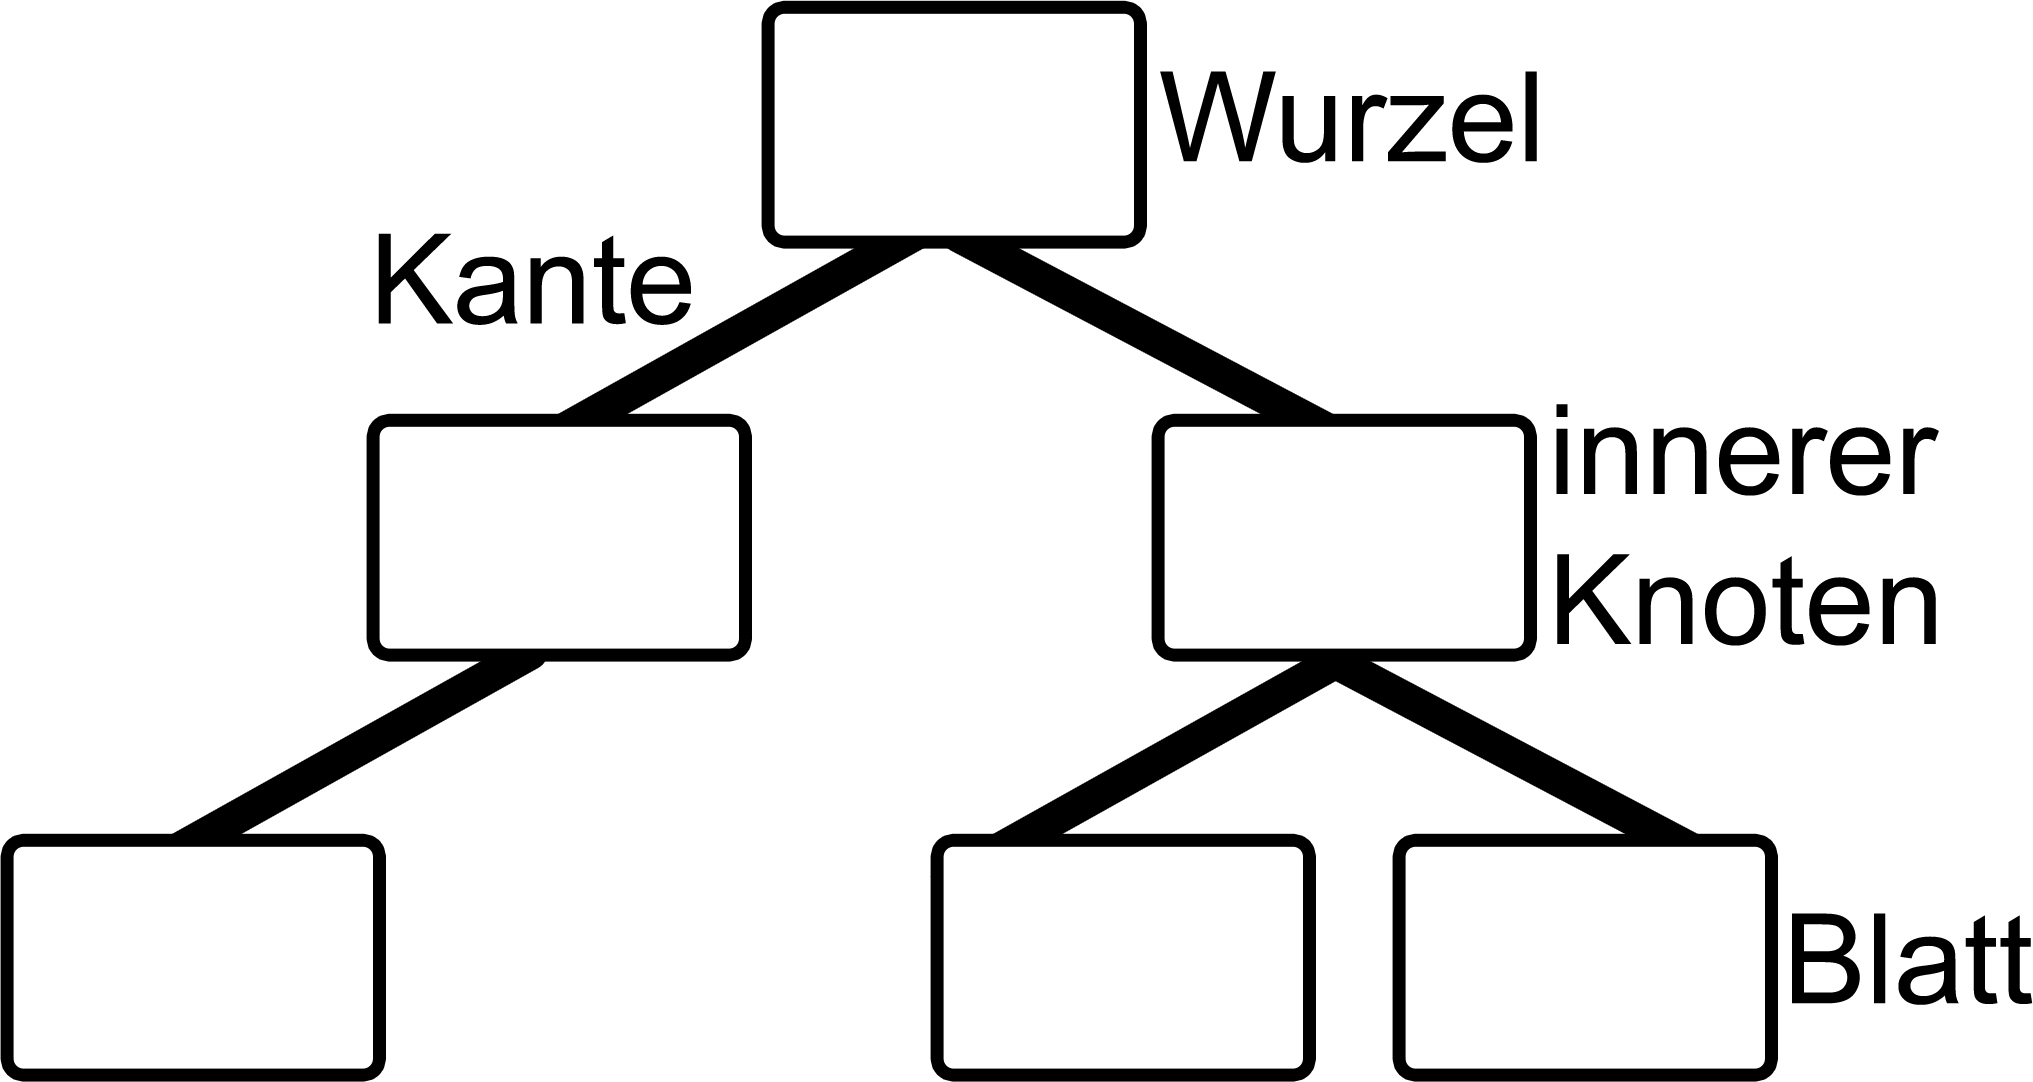
\includegraphics[width=\linewidth]{images/binarytree.jpg}
  \caption{Baumstruktur}
  \captionsource{Von Mhombach - Eigenes Werk, CC BY-SA 3.0, https://commons.wikimedia.org/w/index.php?curid=29981537}
  \label{fig:binarytree}
\end{figure}

Eine Baumstruktur (\ref{fig:binarytree}) besteht aus einem Wurzel-knoten,
welcher mithilfe von Kanten ``Kindknoten'' oder auch ``innere Knoten'' besitzen
kann. Hat ein Knoten keine ``Kinder'', wird er als ``Blatt'' bezeichnet.
Baumstrukturen sind für die Darstellung von Daten aufgrund ihrer einfachen
Gestaltung vorteilhaft. Eine Baumstruktur kann sehr leicht mithilfe von
rekursiven Funktionen durchlaufen werden, da ein Knoten immer genau ein
``Elternteil'' und eine Liste von ``Kindern'' hat.

\section{\acl{VDOM}}
\subsection{Definition}

Ein \ac{VDOM} ist eine Repräsentation eines \ac{DOM} welche durch arbiträre
Datenstrukturen abgebildet werden kann. Eine häufige Implementation ist durch
Javascript-Objekte, welche die Daten des \ac{DOM} abbilden.

\subsection{Motivation}

Oft wird ein \ac{VDOM} verwendet, da aus manipulation der Daten automatisch eine
Änderung im \ac{DOM} abgebildet werden kann, und somit der Entwickler lediglich
die Änderung der Daten bedenken muss.

\subsection{Nachteile}

Eine Repräsentation des \ac{DOM} als \ac{VDOM} führt zwangsläufig dazu, dass die
Struktur des \ac{DOM} doppelt vorhanden ist. Desweiteren ist das finden der
Änderungen zwischen \ac{DOM} und \ac{VDOM} nicht trivial und langsamer als eine
``direkte'' Änderung der Daten im \ac{DOM}. Weiterhin muss der Web-Browser
zusätzlich zum finden der Änderungen zwischen \ac{DOM} und \ac{VDOM} immer
die \ac{DOM}-\ac{API} Aufrufe ausführen.

\section{Statemanagement}
\subsection{Repräsentation}
\subsection{Änderungen}
\section{\acl{SPA}}
Eine \ac{SPA} beschreibt eine Web-Applikation, die auf einer Webseite abgebildet ist. Dies wird realisiert, indem die gesamte Präsentationslogik, im Kontrast zu traditionellen Webanwendungen, im Browser implementiert wird.\cite{SPA} 
\begin{figure}
  \begin{center}
    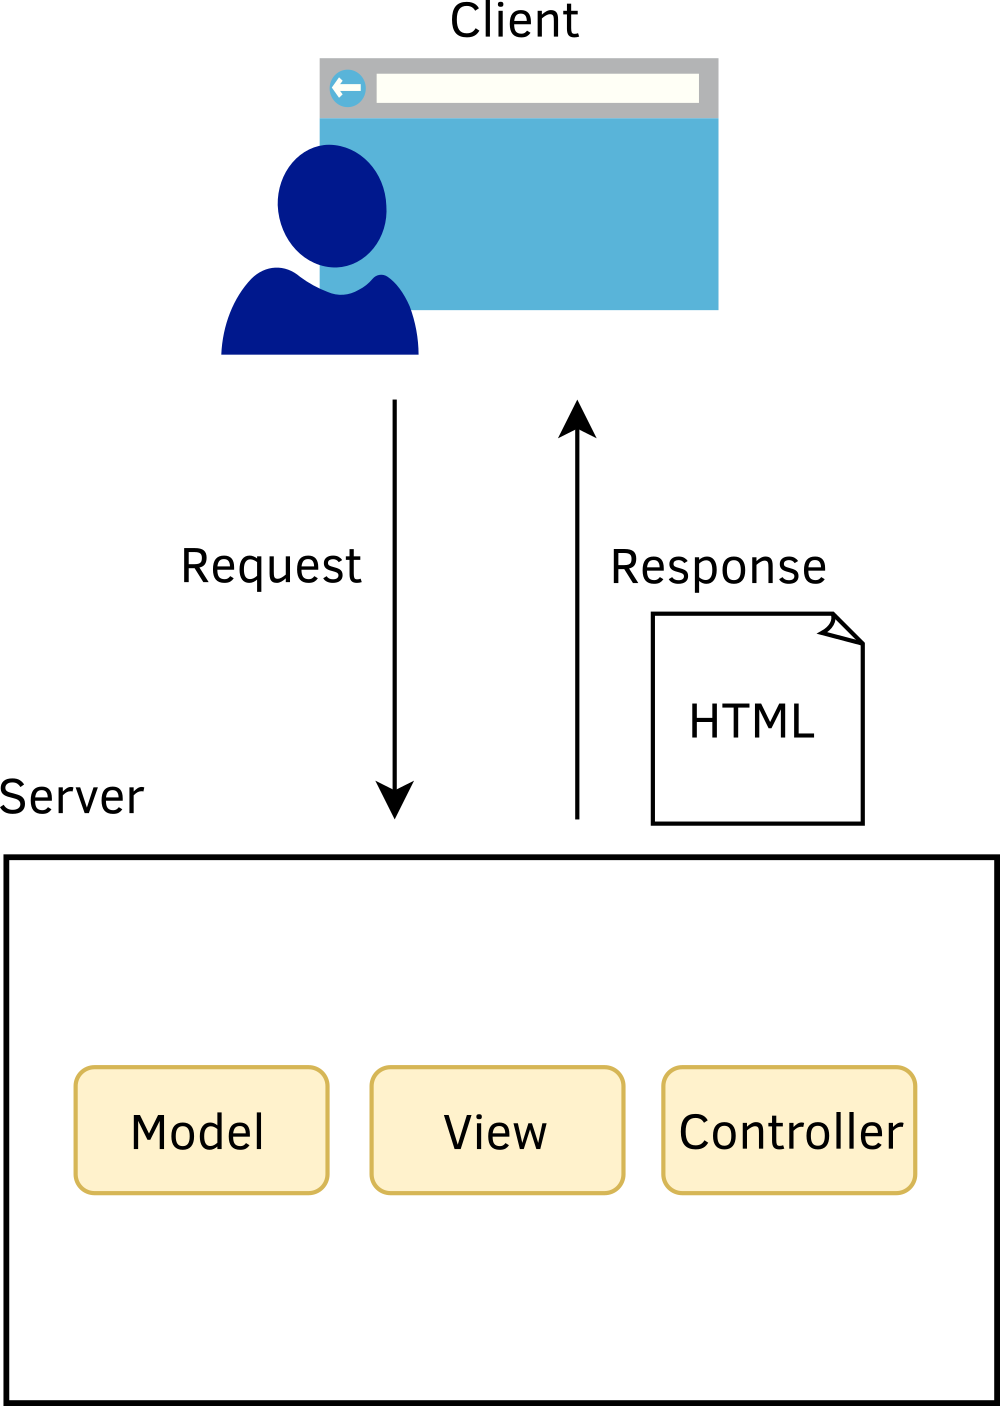
\includegraphics[scale=1]{images/traditonal_web_app.png}
  \end{center}
  \caption{Traditionelle Web Anwendung}
  \captionsource{Eigenes Werk}
  \label{fig:tradweb}
\end{figure}
\subsection{Unterscheidung}
Traditionelle Webanwendungen (siehe Abbildung \ref{fig:tradweb}) lösen bei jeder Anfrage des Nutzers einen Roundtrip \footnote{Senden einer Anfrage an einen Server und Erhalt der entsprechenden Antwort} aus zum Server aus. Serverseitig wird der Request von einem Controller entgegengenommen. Dieser agiert mit dem Model, welches die Daten der Anwendung enthält, und antwortet mit einem neuem \ac{HTML} - Dokument, welches der Browser schließlich anzeigt. Für den Nutzer ist dies durch das aktualisieren der gesamten Webseite sichtbar.

\section{Datenstrukturen}
\subsection{\acl{DBMS}}
\subsection{\acl{ERM}}
\section{\acl{REST}}
\subsection{Definition}
\subsubsection{\acs{REST} Verben}
\section{\acl{RBAC}}
\section{Plugins}
\subsection{Definition}
\subsection{Implementationsansätze}
\subsubsection{Dynamisch}
\subsubsection{Statisch}
% LocalWords:  Superset
